\chapter{Introducción Específica} % Main chapter title

\label{Chapter2}

%----------------------------------------------------------------------------------------
%	SECTION 1
%----------------------------------------------------------------------------------------
En este capítulo se describe en forma global la estructura del sistema y sus funciones. También se establecen los requerimientos y la planificación del proyecto llevado a cabo.

\section{Estructura general del sistema}
Con el objetivo de lograr un sistema adaptable y escalable se optó por realizar un diseño modular. Este diseño consiste en tres tipos módulos o etapas: el módulo principal, los módulos adicionales y la interfaz de usuario. La figura \ref{fig:BloquesGral} indica en forma general la estructura del sistema y el modo en que los módulos están conectados entre sí.


\begin{figure}[ht]
	\centering
	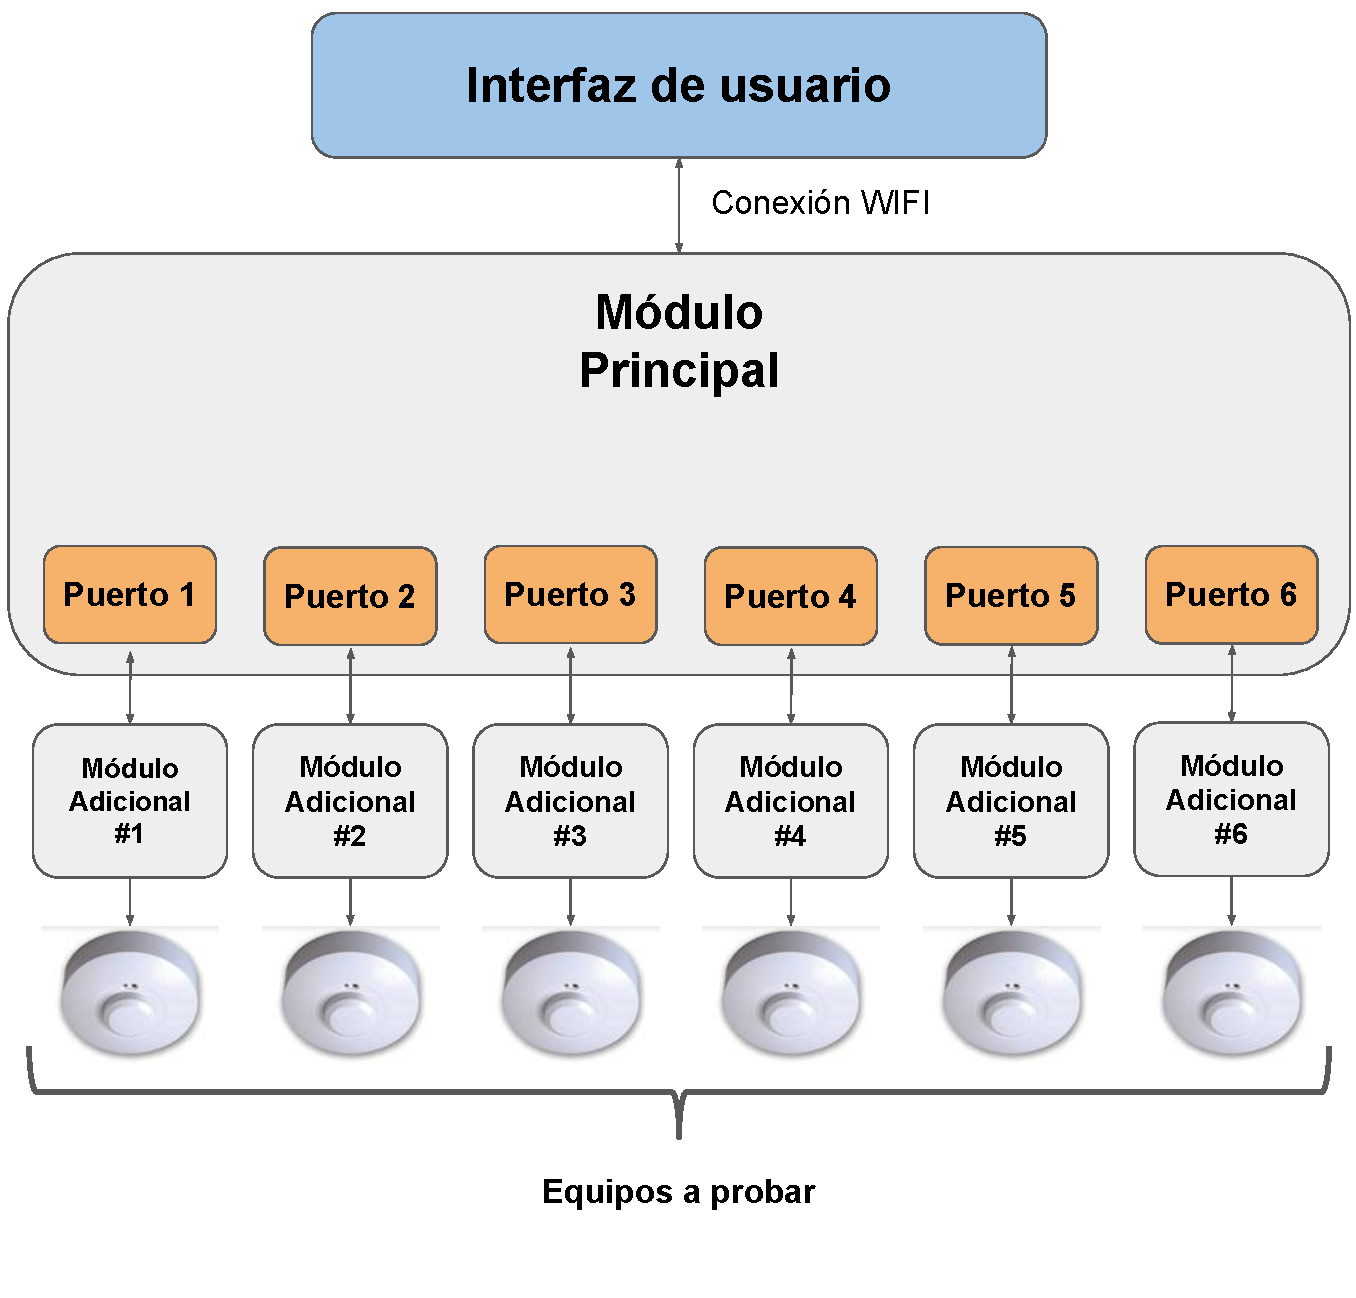
\includegraphics[scale=0.5]{./Figures/BloquesGral.pdf}
	\caption{Diagrama en bloques del sistema.}
	\label{fig:BloquesGral}
\end{figure}

\subsection{Módulo principal}
El módulo principal es la base del sistema, allí se encuentra el núcleo de procesamiento, la etapa de comunicación con la interfaz de usuario, el servidor web de la misma y los puertos de conexión con los módulos adicionales. Estos puertos de conexión son los encargados de capturar las señales provenientes de los módulos adicionales, tanto en forma analógica como digital. Además, son capaces de generar señales analógicas y digitales y proveer de alimentación a los módulos adicionales.
Una característica importante de estos puertos de conexión es que se encuentran aislados eléctricamente uno del otro para poder trabajar con equipos no aislados y únicamente se  comunican con el núcleo de procesamiento mediante una interfaz optoaislada.

\subsection{Módulos adicionales}
Los módulos adicionales cumplen las funciones de conectar y adaptar las señales entre los puertos del módulo principal y el equipo bajo prueba. Estos módulos se diseñan específicamente para cada tipo o familia de productos. Gracias a esta estructura modular se puede adaptar el sistema para realizar distintas pruebas con pocos cambios de hardware.
Al momento se desarrollaron dos módulos adicionales, uno para prueba de temporizadores y otro para la prueba de salida de drivers.

\subsection{Interfaz de Usuario}
La interfaz de usuario es el medio por el cual se controla al sistema. Se desarrolló de forma que pueda ejecutarse en cualquier plataforma que tenga un navegador web y esté conectada a la misma red que el módulo principal. Por ejemplo, se puede ejecutar desde una tablet, notebook o celular y con solo ingresar el IP del sistema de pruebas se tiene acceso al panel de control donde se puede seleccionar la prueba a realizar, configurar los parámetros, ejecutar las pruebas y visualizar los resultados.

\section{Requerimientos}
El diseño del sistema de pruebas se realizó siguiendo una serie de requerimientos que fueron establecidos al comienzo del proyecto. A continuación se detallan cada uno de ellos según la etapa del sistema a la que hacen referencia.

Módulo principal:

\begin{itemize}
	\item Debe poder conectarse a una red WIFI que comparta con la pantalla de usuario.
	\item Debe ser capaz de transmitir información y representarla mediante una interfaz WEB.
	\item Debe ser capaz de recibir órdenes mediante interfaz WEB.
	\item Debe ser posible conectar 6 módulos adicionales del mismo tipo a la vez.
	\item Debe ser capaz de realizar 2 mediciones analógicas simultáneas con una tasa de 	muestreo de al menos mil muestras por segundo.
	\item Debe contar con al menos 3 salidas digitales y 3 entradas digitales por cada puerto. 
	\item Debe disponer de una salida analógica por cada puerto 0-10v.	
	\item Debe poder proveer a los módulos adicionales de alimentación en cada puerto.
	\item Debe poder conectarse con una PC mediante una conexión RS232 a modo de 		puerto de configuración y debugging.
	\item El centro de procesamiento deberá implementarse con un placa EDU-CIAA.
	
\end{itemize}

Módulo adicional para ensayo de Temporizadores:

\begin{itemize}
	\item Debe poder probar temporizadores de 3 y 4 terminales.
	\item Debe proveer de alimentación (220VAC) al equipo bajo prueba.
	\item Debe generar señales que indiquen al módulo principal el estado de funcionamiento del equipo bajo prueba. 
	
\end{itemize}

Módulo para ensayo de driver de luminaria LED:

\begin{itemize}
	\item Debe poder generar señales que indiquen los valores de tensión y corriente de salida del driver bajo prueba.
	\item Debe poder conmutar cargas.
	\item Debe proveer de alimentación (220VAC) al equipo bajo prueba.
	\item Debe proveer al equipo bajo prueba de una señal de control para dimerizado.
\end{itemize}

Control de versiones:

\begin{itemize}
	\item Se debe montar un repositorio GIT.
	\item El repositorio deberá ser accesible mediante la plataforma GITHUB para poder trabajar en forma remota.
\end{itemize}

\section{Planificación}
El desarrollo del sistema de pruebas tuvo como guía la planificación realizada en el marco de la materia gestión de proyectos. Si bien esta planificación original contemplaba que la presentación del prototipo se realizaría en mayo de 2020, fue necesario posponerla debido a que en el momento de realizar las pruebas de las etapas analógicas del módulo principal, se encontró un error de diseño. No pudiendo corregirse este error, fue imperioso agregar una fase de rediseño de las etapas analógicas y la comunicación con los puertos del módulo principal.

